%++++++++++++++++++++++++++++++++++++++++
% Don't modify this section unless you know what you're doing!
\documentclass[letterpaper,12pt]{article}
% \documentclass[onecolumn,conference]{IEEEtran}
\usepackage{tabularx} % extra features for tabular environment
\usepackage{amsmath}  % improve math presentation
\usepackage{graphicx} % takes care of graphic including machinery
\usepackage[margin=1in,letterpaper]{geometry} % decreases margins
\usepackage{cite} % takes care of citations
\usepackage[final]{hyperref} % adds hyper links inside the generated pdf file
\usepackage{hyperref}
\usepackage{amsthm}
\newtheorem{definition}{Definition}[section]
\newtheorem*{remark}{Remark}
\usepackage{booktabs}% for better rules in the table
\usepackage{tabularx}
\setcounter{secnumdepth}{2} % only chapter and sections will be numbered
\setcounter{tocdepth}{3}
\usepackage{caption}
\usepackage{subcaption}
% ++++++++++++++++++++++++++++++++++++++++


\begin{document}

\title{STATS 841: Final Project Report\\Melbourne University Seizure Prediction}

\author{Ruifan Yu \& Shivam Kalra\\\texttt{\{ruifan.yu,shivam.kalra\}@uwaterloo.ca}\\Team: \textit{Overfit}}

\maketitle

\begin{abstract}

We are team \texttt{Overfit} and worked on
\href{https://www.kaggle.com/c/melbourne-university-seizure-prediction}{Melbourne
University AES MathWorks NIH Seizure Prediction}. For the competition, we are
building a model to classify EEG signal into ``Interictal'' or ``Preictal''.
Based on literature review, we are extracting features by FFT, Butterworth
filters and correlation. We are using 3 models to classify EEG. Our first model
is window based with SVM, Gradient Boost and Random Forest as classifiers.
Second is spectrogram based with Convolutional Neural Network (CNN) as
classifier. Third is based on Radon projections with SVM as classifier. Per Kaggle
results, our first model outperformed other two. We've scored \textbf{0.73757}
ranking $\boldsymbol{69^{th}}$ in the public leader-board and \textbf{0.72461}
ranking $\boldsymbol{65^{th}}$ in the private leader-board.

\end{abstract}


\section{Introduction}

Seizure prediction is popular field of research, enabled by statistical analysis
methods applied to features derived from intracranial Electroencephalographic
(EEG) recordings of brain activity~\cite{mirowski2008comparing}. Seizure
forecasting systems have the potential to help patients with epilepsy to lead
more normal lives. For that reason, the Kaggle competition aims at developing a
stable and accurate seizure classifier. In this competition, we are provided
with labeled EEG recordings from 3 patients to train our classification models.
We further use our trained models to predict on the unlabeled testing data,
which is submitted to Kaggle for evaluation.


\subsection{Data Description}

Data for the competition consists of multiple EEG recordings from three
patients. Each recording (known as \textbf{clip}) is 10 minutes long, consisting
of 16 data channels from 16 different electrodes sampled at 400 Hz. Each clip in
training data is categorized as Interictal or Preictal. Number of clips in the
training and testing data for each patient is shown in
Table~\ref{tab:data-summary}. Kaggle uses Area under ROC curve (AUC) as
method of evaluation.

\begin{table}[h]
  \centering
  \begin{tabular}{@{}|l|l|l|l|@{}}
    \toprule
    & \textbf{Patient 1} & \textbf{Patient 2} & \textbf{Patient 3} \\ \midrule
    \textbf{Train} & 1302      & 2346      & 2394      \\ \midrule
    \textbf{Test}  & 216       & 1002      & 690       \\ \bottomrule
  \end{tabular}
  \caption{Number of data clips in train and test data-sets for each patient.\label{tab:data-summary}}
\end{table}

\subsection{Problems in Data-set}
By analyzing the data-set, we found two major issues that influences
the training of our models.

\begin{enumerate}
\item \textbf{Categorical Imbalance:} Number of positive (preictal) and
  negative (interictal) samples are highly unbalanced. It
  decreases the recall rate and results in high false negative rate when
  proper regularization/preventive measures are not applied.

\item \textbf{Random Dropouts:} Some portion of clips have random dropouts (all
  zeros). In some rare cases, clips are entirely empty. This brings
  noise to our classifiers and further influences their accuracy.
  
\end{enumerate}

\section{Feature extraction}\label{sec:feat}

All our feature extractions rely on 6 useful frequency intervals as mentioned in
\cite{howbert2014forecasting}: Delta (0.1 -- 4 Hz), Theta (4 -- 8 Hz), Alpha (8
-- 12 Hz), Beta (12 -- 30 Hz), Lowgamma (30 -- 70 Hz) and Highgamma (70 -- 180
Hz). We are using four kinds of features to train our models as
summarized in Table~\ref{tab:features}.

% Please add the following required packages to your document preamble:
% \usepackage{booktabs}
\begin{table}[ht]
  \centering
  \begin{tabularx}{\textwidth}{@{}|l|X|l|@{}}
    \toprule
    \textbf{Domain}  & \textbf{Feature}                         & \textbf{Used By}   \\ \midrule
    Frequency Domain & Mean \& Variance of magnitudes in six frequency bands  & Model 1            \\ \midrule
    Time Domain      & Mean power ($amplitude^2$) for six frequency bands & Model 1            \\ \midrule
    Time Domain      & Pairwise correlations among 16 channels              & Model 1            \\ \midrule
    Frequency Domain & Spectrograms (binned in frequency and time domain)                             & Model 2 \& Model 3 \\ \bottomrule
  \end{tabularx}
  \caption{Different features extracted in different domains for training models. \label{tab:features}}
\end{table}

We apply Fast Fourier Transform to channel's data for collecting the magnitude
information in all six frequency bands. We also use Butterworth band pass filter
to extract average power ($amplitude^2$) in the time domain for
all six frequency bands. Then we extract pair-wise correlation channels in
time domain, as in \cite{mirowski2009classification}. All these features are
extracted from a \textit{window} (see Def~\ref{def:window}). Spectrograms are non-windowed, however we
still apply binning in time and frequency domain to make them more useful
(used by Model 2 \& Model 3).

\begin{definition}\label{def:window}{Window:} A non-overlapping sub-sample from the clip in all 16
channels.\end{definition} We tried different window size such as: 5, 10,
20 and 60 seconds for the training purposes. Window enables down-sampling of the data and
filtration of the noise \& dropout areas.

TSNE is a technique to visualize the manifolds in higher dimensional data in low
dimension (for example 2D or 3D). Figure~\ref{fig:tsne} shows the separability of
different features extracted for different models. We can see that features for
window based model are better distributed for the classification task which is
evident from the results discussed in later sections.

\begin{figure}[] \centering
	\begin{subfigure}[t]{2in} \centering
    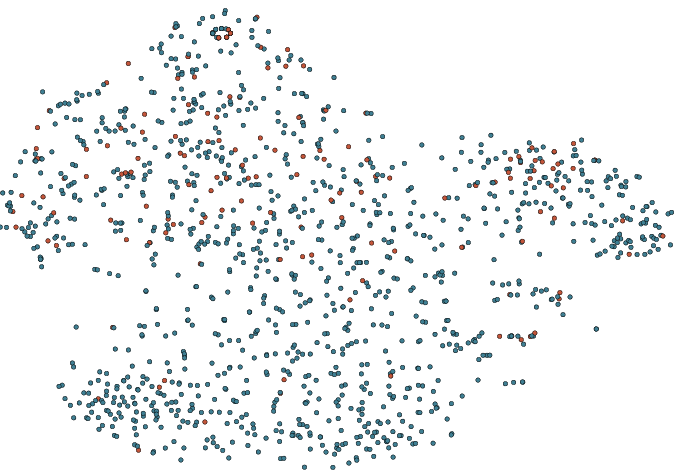
\includegraphics[scale=0.2]{images/tsne_raw_data.png}
		\caption{Raw channel data}\label{fig:1a}
	\end{subfigure}
 	\begin{subfigure}[t]{2in} \centering
    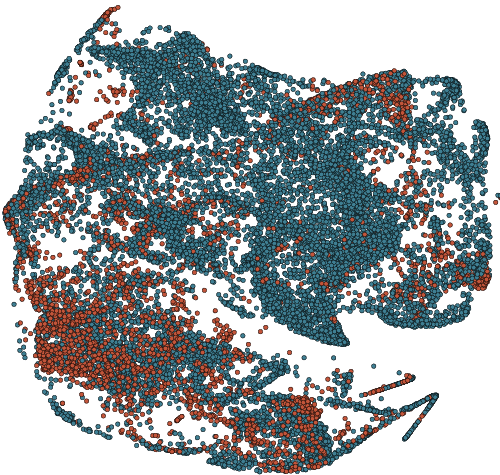
\includegraphics[scale=0.2]{images/trad_feat_viz.png}
		\caption{Window features}\label{fig:1b}
	\end{subfigure}
  \begin{subfigure}[t]{2in} \centering
    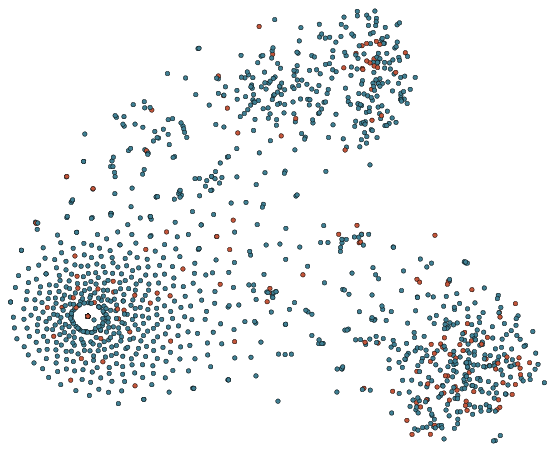
\includegraphics[scale=0.2]{images/tsne_Radon.png}
		\caption{Radon features}\label{fig:1b}
	\end{subfigure}
	\caption{TSNE visualization of features (blue is interictal and red is
    preictal) from (a) raw channel data, (b) features from windows based model and
    (c) radon features}\label{fig:1}
  \label{fig:tsne}
\end{figure}

\section{Models}
Since seizure activity is highly individual, we train one model per patient.
Following section explains details of three of our models.

\subsection{Window Based Model}

\subsubsection{Motivation} 
SVM, Gradient Boost and Random Forest are well suitable for binary
classification with hand-crafted features. Therefore, we used them as
the classifiers in our first model which is based on features extracted from
\textit{window}. We call this model as \textbf{Window based model}.


\subsubsection{Design}
As shown in Figure~\ref{fig:m1}, window based model consists of three parts: 1)
Feature extraction, 2) Training and 3) Prediction using aggregation. In the feature
extraction step, we extract the features according to the
Table~\ref{tab:features}. For collecting data to train classifiers, we randomly select
$20$ windows per \textbf{clip} and extract feature of size $408$ per
\textbf{window}.


\begin{figure}[h]
  \centering
    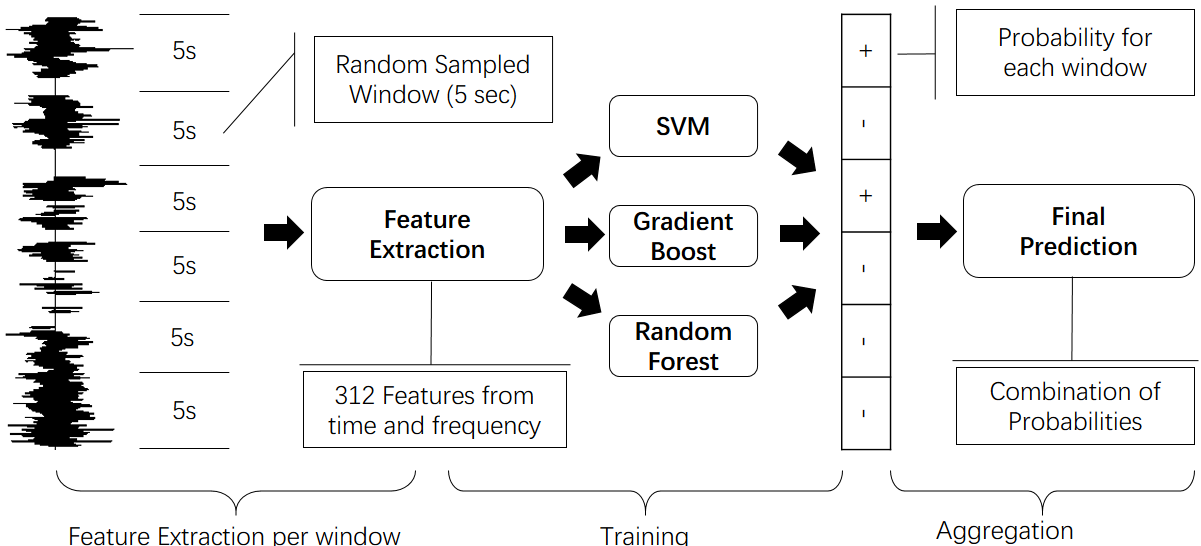
\includegraphics[width=0.74\textwidth]{images/m1.png}
  \caption{Window Based model.}
  \label{fig:m1}
\end{figure}
Then, we feed our classifiers with all the training data. By our design, instead
of directly predicting the final probability, this model will first predict the
probability for each window then generate a final probability by aggregating the
predictions for all windows (refer to Figure~\ref{fig:m1}). Ideally, this may
bring more robustness to our model.

% \subsubsection{Implementation}
% Our solution for this model is implemented using \texttt{Python}. For SVM and
% Random Forest we are using \texttt{Scikit-Learn} library. For Gradient Boosting,
% we used \texttt{XGBoost} library.

\subsubsection{Analysis}\label{sec:ruifan_analysis}
Through experiments, we found that unbalanced data lead to bad
recall rate. Although the general AUC score was good in cross-validation set, we
were not doing well in detecting ``Preictal'' cases. Besides, since we did not know the
ratio in test data, we should focus more on the sensitivity. Therefore, we did
some tuning works on parameters to fix these problems.

Data is unbalanced, therefore, we manually set a bigger weight to the positive
samples penalizing misclassified positive observations, henceforth brings the better
results.

As for the AUC score, we found an interesting issue that we could not get a
accurate estimation of our model. Even though the model performed so well in
cross-validation set, the Kaggle score was much lower. After some analysis, we
realized that this was caused by shuffling and splitting the train--test
data-set.

Some 10 min clips may come from same hour segment and they are very similar.
Therefore, the window features extracted from these clips could be similar too.
After we created the cross-validation set, there were some observations that
were identical to some others in training set. It is a kind of data leakage. As
the data is time-series, it needs some tricks to set up the suitable test set.
After being aware of that, we manually selected test data set so that there was
no overlapping between the train--test data sets.

Over-fitting is very common for this kind of unbalanced data-set. In order to
reduce the influence of over-fitting, we added many methods to punish the
complexity of our model. In SVM, we limited the flexibility of decision
boundary, giving us less penalty to wrong predictions. For Gradient Boost, we
limited the max depth of decision tree, the min child weight and running
iterations. Besides, during training, instead of using full train set, we
randomly sub-sampled the data-set to introduce more robustness to our model.

\subsection{Spectrogram based model}
\subsubsection{Motivation}
Convolutional Neural Network (CNN) has been used in seizure detection in various studies, for
ex.~\cite{mirowski2009classification,korshunova_faculty_2015}. These studies
have shown that CNN is a very competitive method for seizure prediction,
meanwhile CNN is state-of-art in computer vision domain nowadays.

\subsubsection{Design}
We generate spectrograms for each channel with 60 time bins and 6 frequency
bins. 6 frequency bins are selected  as mentioned earlier in
Section~\ref{sec:feat}. 60 time bins are equal sized windows of 10 seconds each.
Since there are 16 channels, we get (16 x 6 x 60) image for each clip (first
dimension is channel depth and (6 x 60) is resolution of image).

With spectrogram, the prediction is turned into image classification problem. The architecture
of CNN that results in best AUC score is shown in Figure~\ref{fig:cnn}.

\begin{figure}[h]
  \centering
    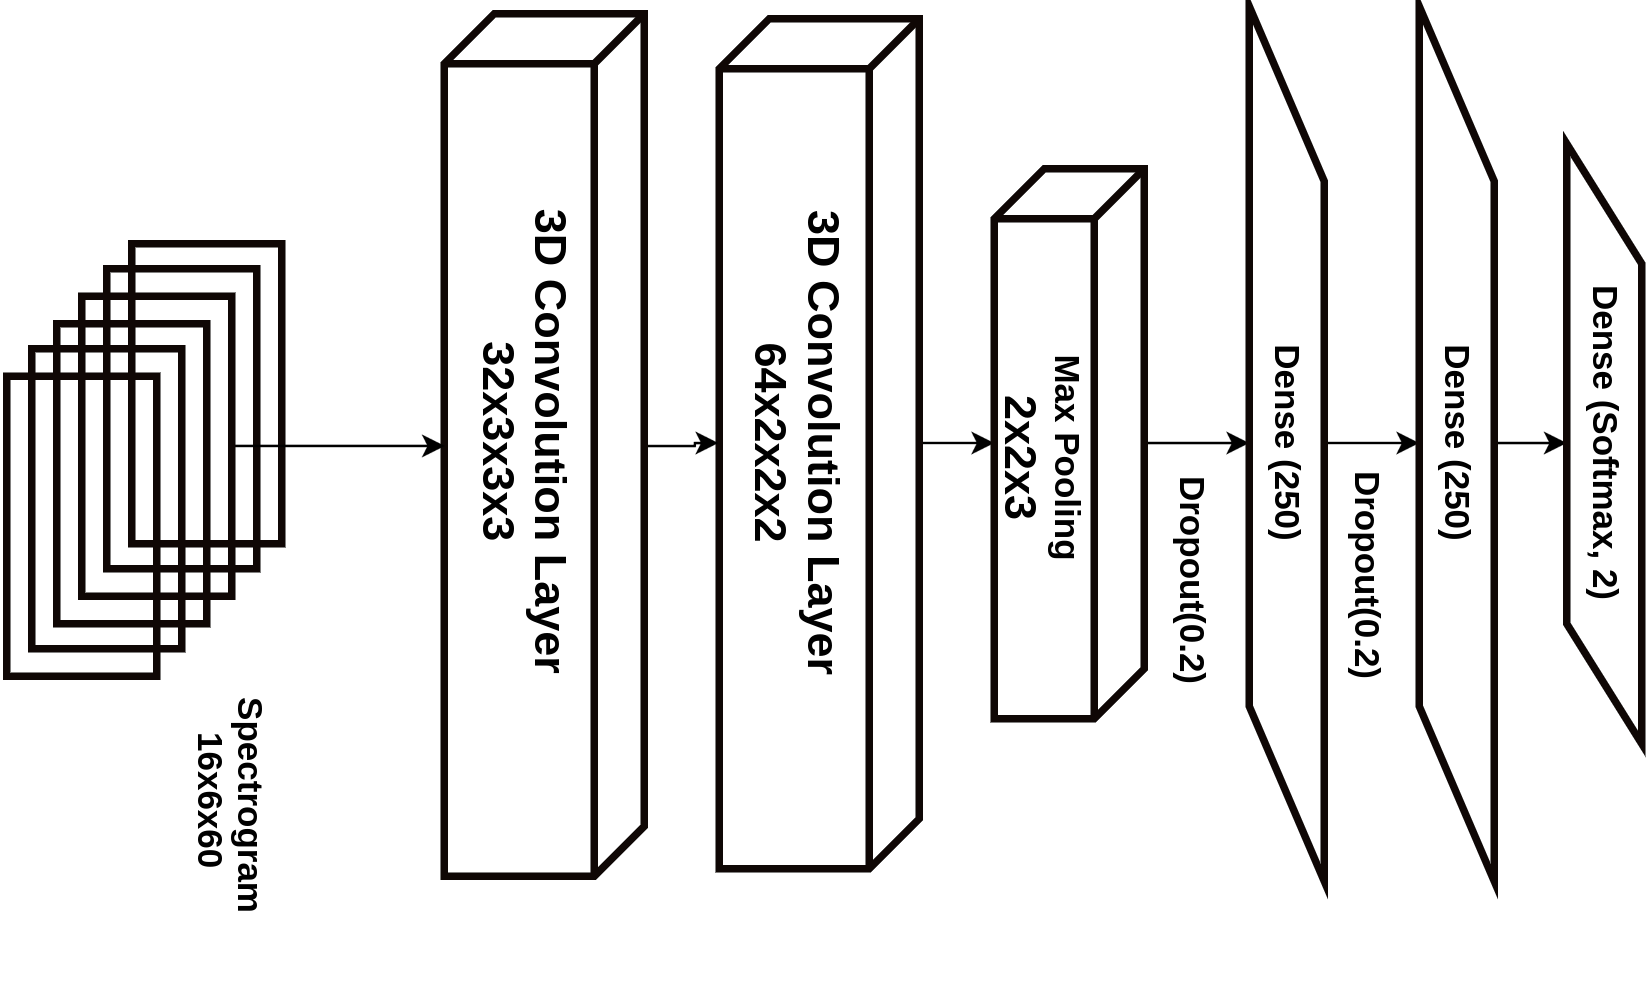
\includegraphics[width=0.8\textwidth]{images/cnn.png}
  \caption{Architecture of CNN using 3D convolution kernels.}
  \label{fig:cnn}
\end{figure}

% \subsubsection{Implementation}
% CNN is implemented in \texttt{Python} using \texttt{Theano}, \texttt{TensorFlow}
% and \texttt{Keras} libraries.

\subsubsection{Analysis}
Problem of unbalanced data and random dropouts is solved using data
augmentation. Data augmentation enables us to create extra data during training
phase. We regularize our CNN predictor by adding the dropout
layers~\cite{srivastava2014dropout}, which prevent the over-fitting.


\subsection{Radon projections based model}

\begin{definition}{Radon Transform} adds up the pixel values in the given image
  along a straight line in a particular direction and at a specific displacement.
\end{definition}

\subsubsection{Motivation}
In existing literature, Radon transform has been used on spectrograms to extract
the effective acoustic features from the speech
data\cite{ajmera_text-independent_2011-2}. It is vastly studied and
reputed feature extraction technique in computational
medicine. It forms basis of CT scans, tomography
and used in compression of medical images.

\subsubsection{Design}
For every clip, spectrograms (16x10x60) are stacked in vertical direction to
create a single spectrogram (160x60) called \textbf{stitched spectrogram}.
Stitched spectrogram is used to calculate the Radon projections from 16
equidistant angles (between $0^\circ$ -- $180^\circ$), giving 2D vector of
16x171 as a feature. These 2D features are flattened into 1D vector (size of
2763) which are subsequently used to train SVM classifier.

\begin{figure}[h]
  \centering
    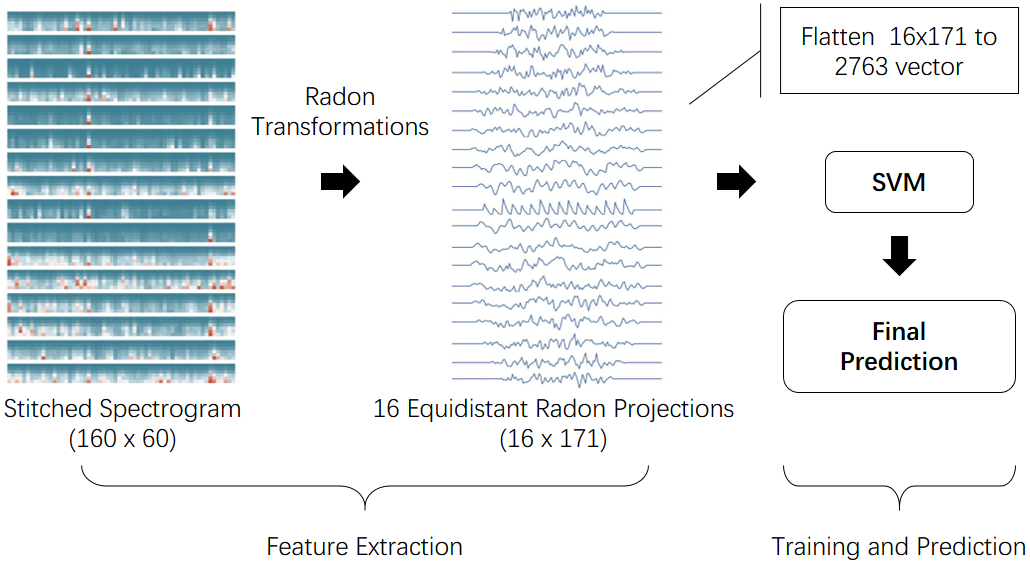
\includegraphics[scale=0.5]{images/radons.png}
  \caption{Overview of the Radon Projections based model.}
  \label{fig:radon_overview}
\end{figure}

% \subsubsection{Implementation}
% We implemented our solution for the model in \texttt{Python} using \texttt{Scikit-Learn}
% and \texttt{Scikit-Image} libraries.

\subsubsection{Analysis}
Keeping unbalanced labels in mind, we trained SVM with more emphasis on positive
cases (preictal). We trained using 5-fold cross validation to prevent wrongful
learning due to data dropouts. Other problems and their solutions during
the training of SVM have been discussed in previous
Section~\ref{sec:ruifan_analysis}.

\section{Results}

Table~\ref{tab:results} shows our Kaggle scores for submissions using different models. We are
not surprised to see that Model 1 out-performed from all models. For
the spectrogram based model, we suffered over-fitting. It also shows that
Radon transformation based model is not suitable for this data-set. We tried
some modifications not no improvement in Radon model.

\begin{table}[h]
  \centering
  \begin{tabular}{@{}lll@{}}
    \toprule
    \textbf{Model}                 & \textbf{Public Leader-board} & \textbf{Private Leader-board} \\ \midrule
    \multicolumn{1}{|l|}{Model 1}  & \multicolumn{1}{l|}{0.69443} & \multicolumn{1}{l|}{0.74115}  \\ \midrule
    \multicolumn{1}{|l|}{Model 2}  & \multicolumn{1}{l|}{0.71466} & \multicolumn{1}{l|}{0.64398}  \\ \midrule
    \multicolumn{1}{|l|}{Model 3}  & \multicolumn{1}{l|}{0.65910} & \multicolumn{1}{l|}{0.65460}  \\ \midrule
    \multicolumn{1}{|l|}{Average Ensemble} & \multicolumn{1}{l|}{0.73757} & \multicolumn{1}{l|}{0.67062}  \\ \midrule
    \multicolumn{1}{|l|}{Ensemble (Weighted)}            & \multicolumn{1}{l|}{0.70371}                      & \multicolumn{1}{l|}{0.72461}                       \\ \bottomrule
  \end{tabular}
  \caption{Kaggle scores from all three models (including two ensembles) \label{tab:results}}
\end{table}

We selected average ensemble and weighted ensemble as our two submissions for
the final evaluation.

\begin{remark} Our team \textbf{Overfit} scored \textbf{0.67062} ranked at
$158^{th}$. However, our last submission was made using account
\textbf{RuifanYu} scoring \textbf{0.72461} ranking $65^{th}$. Since we have
access to all our final private leader-board scores, our best entry scored
\textbf{0.74115} by Model 1 (without ensemble).
\end{remark}

  
\section{Conclusions}
During this project, we learned a lot in application of machine learning and how
handle parameter tuning and large data-sets. In real world scenarios, the
feature engineering is the most important aspect. From this project, we also
realize that deep learning is not very suitable for every kind of problem. So
far, tree-based classifiers and SVM are still the dominant methods, they balance
out well between over-fitting and under-fitting and are usually significantly
faster than training deep neural networks.

\begin{remark} Source codes/presentation can be accessed at:
  \href{https://github.com/shivamkalra/stats-841-project}{Github Repository}
\end{remark}

\bibliographystyle{acm}
\bibliography{ref}

\end{document}
